\section{Proposed Outline}

- define outline
- Preface
    - Acknowledgement
    - Bookmanager
- Introduction
    - What this is doing
    - Why it matters
    - Related Research
        - List references
        - Explain what others have done
- Installation
    - Python virtual environment
    - Installation of mpi4py
    - Installation of NumPy and Jax
    - Cloudmesh
        - Cloudmesh.StopWatch
- Sequential sorting
    - Overview of sequential sorting algorithms
    - Algorithms/implementations
        - Sequential merge sort
        - Insertion sort
        - Bubble sort
        - Quick sort
- Parallel sorting
    - Related algorithms
        - Bitonic sort
    - Multiprocessing merge sort
    - MPI merge sort
        - MPI builtin merge sort
        - MPI sequential merge sort
        - MPI adaptive merge sort
            - One way bitonic sort?
- Sorting on GPU
    - Jax NumPy
- Performance comparision
- Visualization
    - Automated Jupyter notebooks for performance comparison
- Conclusion

\section{Preface}

\section{Introduction}

\section{Installation}

\section{Sequential Sorting}

\subsection{Recursive Merge Sort}

Recursive merge sort is a standard example of a divide-and-conquer algorithm. The algorithm can be split into two parts:
splitting and merging.

Merging describes the merging of two sorted lists into one sorted list. Two ways of doing so are described below.

**Method 1: Iterative Method**

Assign indexes to the beginning of each array. Check for the smaller of each element at the current index and add it to
the end of the sorted list. Increment the index of the list whose number was found. Once one array is empty, we can
simply append the other one onto the end of the sorted list.

\begin{verbatim}
python3 code to demonstrate merging two sorted lists using the iterative method

right = [1, 2, 6, 7, 15]
left = [3, 4, 5, 8, 13]

res = []
left and right indexes
i, j = 0, 0

while i < len(left) and j < len(right):
    find the smallest value at either index 
    and append it to the sorted list
    if left[i] < right[j]:
        res.append(left[i])
        i += 1
    else:
        res.append(right[j])
        j += 1

at least one array is empty
append both onto the end of the sorted list
res = res + left[i:] + right[j:]
\end{verbatim}

**Method 2: Using *sorted()***

By using the built-in Python function *sorted()*, we can merge the two lists in one line.

\begin{verbatim}
right = [1, 2, 6, 7, 15]
left = [3, 4, 5, 8, 13]

concatenate and sort
res = sorted(left + right)
\end{verbatim}

Once we can merge two sorted arrays, the rest of mergesort follows as such:

Given an array of length n,

1. If n > 1, divide the array into two halves, or subarrays;
2. Use mergesort to sort each of the two subarrays;
3. Merge the two sorted subarrays into one sorted array.

\begin{verbatim}
def sequential_mergesort(array):
    n = len(arr)
    if n > 1:
        left = array[:n / 2]
        right = array[n / 2:]

        sequential_mergesort(left)
        sequential_mergesort(right)

        merge(left, right)
\end{verbatim}

A variant on this approach is to stop splitting the array once the size of the subarrays gets small enough. Once the
subarrays get small enough, it may become more efficient to use other methods of sorting them, like the built-in
Python *sorted()* function instead of recursing all the way down to size 1.

\begin{verbatim}
def sequential_mergesort(array):
    n = len(arr)
    if n < SMALLEST_ARRAY_SIZE:
        array = sorted(array)
        return

    left = array[:n / 2]
    right = array[n / 2:]

    sequential_mergesort(left)
    sequential_mergesort(right)

    merge(left, right)
\end{verbatim}

The average time complexity of classic merge sort is O(n logn), which is the same as quick sort and heap sort.
Additionally, the best and worst case time complexity of merge sort is also O(n log n), which is the also same as quick
sort and heap sort. As a result, classical merge sort is generally unaffected by factors in the initial array.

However, classical merge sort uses O(n) space, since additional memory is required when merging. Quicksort also has this
space complexity, while heap sort takes O(1) space, since it is an in-place method with no other memory requirements.
\begin{comment}
\begin{table}[!ht]
    \centering
    \begin{tabular}{|l|l|l|l|}
    \hline
        Sort & Average Time Complexity & Best Time Complexity & Worst Time Complexity \\ \hline
        Bubble sort & $O(n^2)$ & O(n) & O(n\^2) \\ \hline
        Insertion sort & O(n\^2) & O(n) & O(n\^2) \\ \hline
        Selection sort & O(n\^2) & O(n\^2) & O(n\^2) \\ \hline
        Heap sort & O(nlogn) & O(nlogn) & O(nlogn) \\ \hline
        Quick sort & O(nlogn) & O(nlogn) & O(nlogn) \\ \hline
        Merge sort & O(nlogn) & O(nlogn) & O(nlogn) \\ \hline
    \end{tabular}
\end{table}
\end{comment}
\section{Parallel Sorting}

Parallel programming describes breaking down a task into smaller subtasks that can be run simultaneously. Since merge
sort is a classic and well-known example of the divide-and-conquer approach, we use merge sort as a test method to
explore parallelization methods that may be generalizable to other divide-and-conquer methods.

\subsection{Related Research}

The theory of merge sort parallelization has been studied in the past. Cole (1998) presents a parallel implementation of
the merge sort algorithm with O(log n) time complexity on a CREW PRAM, a shared memory abstract machine which neglects
synchronization and communication, but provides any number of processors. Furthermore, Jeon and Kim (2002) explore a
load-balanced merge sort that evenly distributes data to all processors in each stage. They achieve a speedup of 9.6
compared to a sequential merge sort on a Cray T3E with their algorithm.

On MPI, Randenski (2011) describes three parallel merge sorts: shared memory merge sort with OpenMP, message passing
merge sort with MPI, and a hybrid merge sort that uses both OpenMP and MPI. They conclude that the shared memory merge
sort runs faster than the message-passsing merge sort. The hybrid merge sort, while slower than the shared memory merge
sort, is faster than message-passing merge sort. However, they also mention that these relations may not hold for very
large arrays that significantly exceed RAM capacity.

\url{https://www.researchgate.net/publication/220091378_Parallel_Merge_Sort_with_Load_Balancing}

\url{http://www.inf.fu-berlin.de/lehre/SS10/SP-Par/download/parmerge1.pdf}

\url{https://charm.cs.illinois.edu/newPapers/09-10/paper.pdf}

\subsection{Multiprocessing Merge Sort}

*multiprocessing* is a package that supports, on Windows and Unix, programming using multiple processors on a given
machine. Python's Global Interpreter Lock (GIL) only allows one thread to be run at a time under the interpreter, which
means multithreading cannot be used when the Python interpreter is required. However, the *multiprocessing* package
side-steps this issue by using subprocesses instead of threads. Because each process has its own interpreter with a
separate GIL that carries out its given instructions, multiple processes can be run in parallel.

The docs for the *multiprocessing* package can be read [here](https://docs.python.org/3/library/multiprocessing.html).

\subsubsection{Overview}

We use Python to implement a multiprocessing mergesort algorithm
(linked: \href{https://github.com/cloudmesh/cloudmesh-mpi/blob/main/examples/sort/multiprocessing_mergesort.py}{here}. The
algorithm is then run and evaluated
in \href{https://github.com/cloudmesh/cloudmesh-mpi/blob/main/examples/sort/sandra.ipynb}{here}.

\subsubsection{Algorithm}

We define a merge function that supports explicit left/right arguments, as well as a two-item tuple, which works more
cleanly with multiprocessing. We also define a classic merge sort that splits the array into halves, sorts both halves
recursively, and then merges them back together.

Once both are defined, we can then use multiprocessing to sort the array.

First, we get the number of processes and create a pool of worker processes, one per CPU core.

\begin{verbatim}
processes = multiprocessing.cpu_count()
pool = multiprocessing.Pool(processes=processes)
\end{verbatim}

Then, we split the intial given array into subarrays, sized equally per process, and perform a regular merge sort on
each subarray. Note that all merge sorts are performed concurrently, as each subarray has been mapped to an idividual
process.

\begin{verbatim}
size = int(math.ceil(float(len(data)) / processes))
data = [data[i * size:(i + 1) * size] for i in range(processes)]
data = pool.map(merge_sort, data)
\end{verbatim}

Each subarray is now sorted. Now, we merge pairs of these subarrays together using the worker pool, until the subarrays
are reduced down to a single sorted result.

\begin{verbatim}
while len(data) > 1:
    extra = data.pop() if len(data) % 2 == 1 else None
    data = [(data[i], data[i + 1]) for i in range(0, len(data), 2)]
    data = pool.map(merge, data) + ([extra] if extra else [])
\end{verbatim}

If the number of subarrays left is odd, we pop off the last one and append it back after one iteration of the loop,
since we're only interested in merging pairs of subarrays.

Entirely, the parallel merge sort looks like this:

\begin{verbatim}
def merge_sort_parallel(data):
    processes = multiprocessing.cpu_count()
    pool = multiprocessing.Pool(processes=processes)

    size = int(math.ceil(float(len(data)) / processes))
    data = [data[i * size:(i + 1) * size] for i in range(processes)]
    data = pool.map(merge_sort, data)

    while len(data) > 1:
        extra = data.pop() if len(data) % 2 == 1 else None
        data = [(data[i], data[i + 1]) for i in range(0, len(data), 2)]
        data = pool.map(merge, data) + ([extra] if extra else [])

    return data[0]
\end{verbatim}

\subsection{MPI Merge Sort}

BOGO describe MPI
MPI for Python, also known as mpi4py, is an object oriented approach to message passing in Python. It closely follows
the MPI-2 C++ bindings.

[Linked](https://mpi4py.readthedocs.io/en/stable/index.html)

\subsubsection{Overview}

This project uses Python to implement an MPI mergesort algorithm (linked
%[here](https://github.com/cloudmesh/cloudmesh-mpi/blob/main/examples/sort/night.py)).
The algorithm is then run and evaluated in
%[mpi_run.py](https://github.com/cloudmesh/cloudmesh-mpi/blob/main/examples/sort/mpi_run.py).

\section{Sorting on GPU}

We measure the performance of our multiprocessing and MPI mergesort algorithms on the Carbonate GPU partition. Each node
is equipped with two Intel 6248 2.5 GHz 20-core CPUs, four NVIDIA Tesla V100 PCle 32 GB GPUs, one 1.92 TB solid-state
% drive, and 768 GB of RAM. We execute our merge sorts with randomly generated arrays of up to 10^7 integer elements. Note
that memory constraints allowed us to experiment with arrays of up to BOGO integer elements.

Multiprocessing merge sort was executed on 1 to 24 processes by using all available processes on the Carbonate partition. Message-passing merge sort was executed on 1, 2, 4, and 8 nodes by using one core on each node for MPI processes. 

\section{Performance Comparison}

All performance comparison done here will be on data from the Carbonate partition. 

\subsection{Time}

Using our results from the Carbonate partition, we analyze and graph the resulting times from selected runs. 

\begin{table}
    \caption{This is an example.}
    \label{tab:times-sort}
    \centering
    % 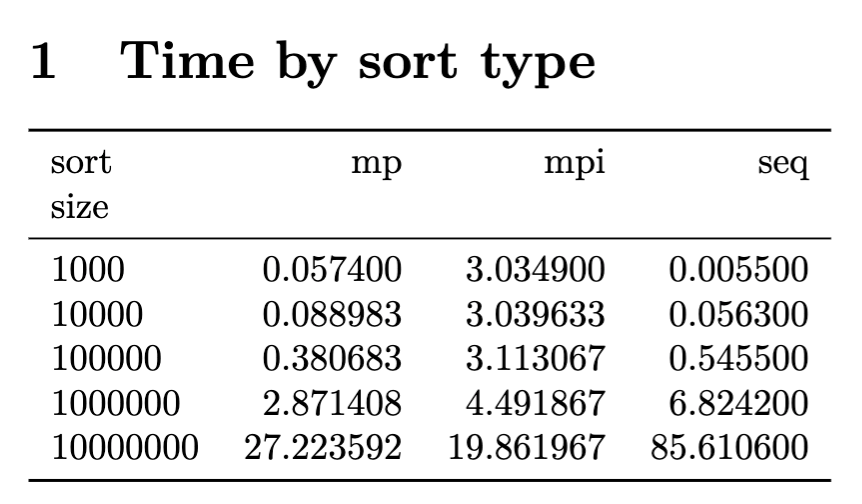
\includegraphics{https://github.com/cloudmesh/cloudmesh-mpi/blob/main/examples/sort/images/time-by-sort-type.png}
    % \begin{tabular}{lrrrrrr}
\toprule
sort &  np-heap &  np-merge &  np-quick &  np-stable &     sort &   sorted \\
size     &          &           &           &            &          &          \\
\midrule
10000000 &   2.2764 &    1.0150 &    0.8018 &     1.0324 &   3.5528 &   3.8602 \\
20000000 &   5.5326 &    2.1080 &    1.6640 &     2.1390 &   8.1444 &   8.2872 \\
30000000 &   9.2384 &    3.3098 &    2.5470 &     3.2274 &  12.8666 &  13.2482 \\
40000000 &  12.9562 &    4.3962 &    3.4990 &     4.4080 &  17.9730 &  20.2934 \\
50000000 &  17.1362 &    5.8164 &    4.4092 &     5.6302 &  24.0766 &  23.3998 \\
60000000 &  21.0888 &    6.8442 &    5.3924 &     6.9958 &  28.7686 &  31.8022 \\
70000000 &  25.0790 &    8.2454 &    6.6280 &     8.2816 &  35.2654 &  37.5924 \\
80000000 &  29.7190 &    9.4926 &    7.2184 &     9.3428 &  39.2304 &  41.7802 \\
\bottomrule
\end{tabular}

\end{table}
% ![Table : Times for different sorts](https://github.com/cloudmesh/cloudmesh-mpi/blob/main/examples/sort/images/time-by-sort-type.png)

We can analyze time in two ways. First, we analyze algorithm performance based on increasing size of arrays. Some algorithms differ within themselves (for example, two multiprocessing merge sorts might use different numbers of processes). However, we can account for this variation by aggregating all the values and showing error bands around the lines that are plotted. 

\begin{figure}
    \centering
    % 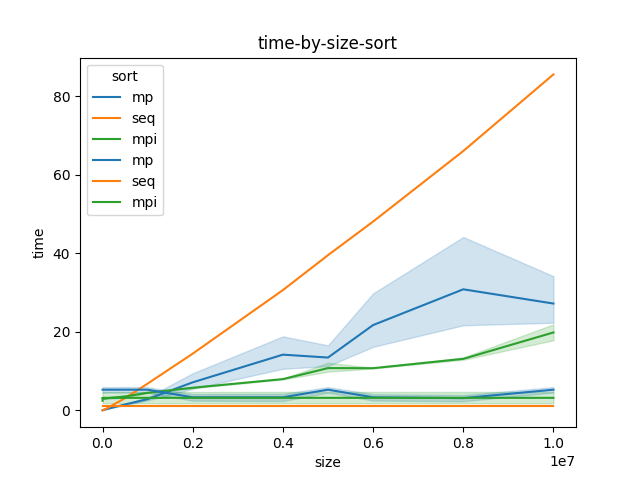
\includegraphics[width=0.5\textwidth,height=\textheight]{https://github.com/cloudmesh/cloudmesh-mpi/blob/main/examples/sort/images/time-by-size-sort.png}
    \caption{Times for different sorts}
    \label{fig:times-sort}
\end{figure}
% ![Fig : Times for different sorts](https://github.com/cloudmesh/cloudmesh-mpi/blob/main/examples/sort/images/time-by-size-sort.png){width="50%"}
\begin{comment}
The figure illustrates the average run time for arrays of up to size $10^7$ for each different sort type (sequential merge sort, multiprocessing merge sort, and MPI merge sort.) 

The general behavior displayed in the figure can be summarized in the following points:
\begin{enumerate}

    \item For array sizes of up to around 2 million, the multiprocessing mergesort, on average, 
    is quicker than the MPI mergesort. The overhead of MPI contributes significantly more to the 
    overall sort time for smaller arrays, since the creation of processes takes longer than the 
    creation of threads. However, the MPI mergesort is consistently the fastest sort type when arrays 
    are sufficiently large enough that the time reduction from parallelism on individual nodes is enough 
    to offset the additional costs of communication and thread creation. 

    \item The MPI sort displays the lowest average increase in time relative for array size, with a mean value of 1.708 seconds/million numbers. In other words, when the array size increases by an additional one million elements, the MPI sort time increases by an average of 1.708 seconds. The multiprocessing sort underperforms this significantly, with a mean increase of 2.706 seconds per additional million numbers. The sequential sort has a mean increase of 8.754 seconds per additional million numbers. 
\end{enumerate}

Second, we analyze algorithm performance based on processes used. We will keep the size of the array at a constant value and, for each number of processes, compare the times for each sorting algorithm. 

![Table x: Time by process for size=10000, mp](https://github.com/cloudmesh/cloudmesh-mpi/blob/main/examples/sort/images/p-time-mp-10000.png)

![Table x: Time by process for size=10000, mpi](https://github.com/cloudmesh/cloudmesh-mpi/blob/main/examples/sort/images/p-time-mpi-10000.png)

![Fig 2: Time by process for size=10000](https://github.com/cloudmesh/cloudmesh-mpi/blob/main/examples/sort/images/time-by-p-sort-10000.png){width="50%"}

For arrays of size 10000, increasing MPI parallelism is actually a positive factor for time. This aligns with what we see above, where MPI mergesort initally performs worse than multiprocessing mergesort on small arrays. 

![Table x: Time by process for size=1e7, mp](https://github.com/cloudmesh/cloudmesh-mpi/blob/main/examples/sort/images/p-time-mp-1e7.png)

![Table x: Time by process for size=1e7, mp](https://github.com/cloudmesh/cloudmesh-mpi/blob/main/examples/sort/images/p-time-mpi-1e7.png)

![Fig 3: Time by process for size=10000000](https://github.com/cloudmesh/cloudmesh-mpi/blob/main/examples/sort/images/time-by-p-sort-10000000.png)

For arrays of size $10^7$, we can see in figure 3 that increasing paralellism reduces runtimes for both algorithms. 

\subsection{Speedup}

Speedup is defined as $\frac{T_s}{T_p}$, where $T_s$ is the compute time of the sequential algorithm and $T_p$ is the compute time of the parallel algorithm. 

\subsection{Efficiency}

\section{Conclusion}

- MPI is advantageous to use when data is large enough
- further speedup can be obtained by using MPI I/O operations. 

\subsection{Source Code}

The source code is located in GitHub at the following location:

- <https://github.com/cloudmesh/cloudmesh-mpi/tree/main/examples/sort>

We distinguish the following important files:

- [night.py](https://github.com/cloudmesh/cloudmesh-mpi/blob/main/examples/sort/night.py)

\subsection{Installation}

\subsubsection{ENV3 (for macOS)}

\end{verbatim} bash
$ python -m venv ~/ENV3
$ source ~/ENV3/bin/activate
\end{verbatim}

\subsubsection{Clone}

To download our code, please follow the instructions:

\end{verbatim} bash
$ mkdir cm
$ cd cm
$ git clone git@github.com:cloudmesh/cloudmesh-mpi.git
\end{verbatim}

\subsubsection{Verification}

Go to the [Github](https://github.com/cloudmesh/cloudmesh-mpi) to verify
that the correct repository has been cloned.

\subsubsection{Updating}

1. Update local version

   \begin{verbatim} bash
   git pull
   \end{verbatim}

2. To add file (only do once)

   \begin{verbatim}
   git add filename
   \end{verbatim}

3. Once file is changed, do

   \begin{verbatim}
   git commit -m "this is my comment" filename
   \end{verbatim}

4. Remote upload

   \begin{verbatim}
   git push
   \end{verbatim}

\subsection{Running the Program}

Run the program using the command

\begin{verbatim}
./mpi_run.py --user={username} --node={node} --sort={mpi_mergesort}--size={size} --repeat={repeat} --id={id}
\end{verbatim}

Please read the Input sectionfor specific documentation on each option.

\subsection{Overview}

This project uses Python to implement an MPI mergesort algorithm (linked
[here](https://github.com/cloudmesh/cloudmesh-mpi/blob/main/examples/sort/night.py)).
The algorithm is then run and evaluated in
[mpi_run.py](https://github.com/cloudmesh/cloudmesh-mpi/blob/main/examples/sort/mpi_run.py).

\subsubsection{Input

*mpi_run.py* has several inputs.

*user*: specify the username of whoever is running the program\
*node*: name of computer node on which program is being run\
*sort*: type of sort that is being run. Use "mpi_mergesort".\
*size*: size of array to sort\
*repeat*: number of times to run sorting algorithm. Final time will be
the average of all runs.\
*id*: specifies the merging algorithm that is used to merge the arrays
once they've been sent from one process to another, also known as the
merge algorithm. Each id number corresponds to a specific algorithm.\
0: built-in Python *sorted*\
1: sequential merge\
2: adaptive merge

For example, if John would like to run the MPI mergesort on his
Raspberry Pi 4, and he would like to use an array of size 200, repeating
10 times, and use an adaptive merge to combine the the arrays between
processes, he would use the command

\begin{verbatim}
./mpi_run.py --user=john --node=pi4 --sort=mpi_mergesort --size=200 --repeat=10 --id=2
\end{verbatim}

\subsubsection{Mergesort

The unsorted array is generated on rank 0. Since the unsorted array must
be split into smaller subarrays, *sub_size* is calculated. *sub_size* is
the size of each subarray. It is equal to the size of the unsorted array
divided by the number of processors, since each processor must be sent a
subarry. Note that *n*, the size of the unsorted array, must be evenly
divisible by the total number of processors.

Once the subarrays have been distributed using the Scatter command, they
are sorted on each processor using the built-in Python. This sort
defaults to Timsort.

In order to merge the sorted subarrays, we can visualize the processors
as being set up in a binary tree, where each parent has two children.
One important note: in this situation, the left child also functions as
the parent node. We can then split the tree into two sections: left
children and right children. Because we are using a binary tree, we know
that the number of left and right children will always be equal.
Therefore, we can create a variable *split* that splits the set of
processors in half.

If the rank of the processor is in the second half (between *split* and
*split* \* 2), then it will send its sorted subarray to its "left"
partner to be merged. Otherwise, if the rank of the processor is in the
first half (between 0 and *split*), it will recieve a sorted subarray
from its "right" partner and then merge it with the subarray that it
currently contains. When a subarray is sent, it is sent to the processor
with rank *rank - split*, ensuring that the processor that it is sent to
has a rank between 0 and *split*. This guarantees that each subarray
that is sent gets sent to a merging processor. Similarly, when a
subarray is received, it is received from a processor with rank *rank +
split*, ensuring that the subarray is a sorted array to be merged. This
mapping guarantees a unique pairing between left and right child.

Once received, the subarrays are merged together. The merging algorithm
can be defined by the user, and will be referred to as the **merge
algorithm**. There are currently three merging algorithms that can be
used. 1. **sequential_merge_fast**, a "fast" merge that simply combines
the two arrays using the built-in Python *sorted* function. Note that
sorting algorithms can also be used to merge. 2.
**sequential_merge_python**, a merge that uses the well-known technique
of appending the smaller of two array elements to a third array 3.
**adaptive_merge**, a custom sort algorithm that takes advantage of
pre-existing order in the sequence. It is described in more detail
[here](sectionadaptive).

Then, each individual send/recieve operates as following:

1. Left child sends sorted subarray
2. Right child allocates memory for recieving subarray from left child
   (*local_tmp*)
3. Right child allocates memory for array to store merged result
   (*local_result*)
4. Right child receives subarray
5. Right child merges received subarray with its own subarray
6. Right child assigns *local_arr* to point to *local_result*

This loop continues until the tree reaches the height that guarantees us
a single sorted list. Each time, the number of nodes is halved (since
two have been merged into one).

\subsubsection{Output

The output of the program is generated and logged in
[mpi_experiment.py](hhttps://github.com/cloudmesh/cloudmesh-mpi/blob/main/examples/sort/mpi_experiment.py).
This file runs the sort according to user specifications. Three of the
most important things it does: 1. The specific algorithm is run *repeat*
times. Note that the larger *repeat* is, the more accurate the final
mean time will be. The mean time is not calculated here. Rather, all
times from each repeat will be outputted. 2. Maps id numbers to merge
types. It's important to be able to differentiate between data outputted
by each merge type, since we'd like to examine the differences. However,
we'd also like to keep the titles/inputs concise, which is why id
numbers are used. Each id number is translated to its merge type in the
program. 3. Times the runs. Running the sort is done by a bash command,
so by starting a timer, running the command, and stopping the timer, we
can get the full amount of time it took to run the sort. This is a more
accurate measure than placing timers inside of the actual sort program
(night.py), since it is able to time the MPI initialization, which
timers inside the program wouldn't be able to do.

\subsubsection{Final Run Method

This is the outermost run program, i.e. the one that a user will run.
See the above Input \section{for an example of how to run this.
[mpi_run.py](https://github.com/cloudmesh/cloudmesh-mpi/blob/main/examples/sort/mpi_run.py)
generates a log file and runs
[mpi_experiment.py](https://github.com/cloudmesh/cloudmesh-mpi/blob/main/examples/sort/mpi_experiment.py).

\subsection{adaptive}

This sort takes advantage of pre-existing sorted subsequences in two
arrays to merge them together. It is designed to merge two sorted arrays
together. Given two arrays, called *left* and *right*, we first
calculate the min and max values in both.

\begin{verbatim}
   l_min = left[0] 
   r_min = right[0]
   l_max = left[len(left) - 1]
   r_max = right[len(right) - 1]
\end{verbatim}

We can also assume that the minimum of left will always be smaller than
the minimum of right (if not, we can just swap them).

The sort splits into three scenarios based on *l_min*, *r_min*, *l_max*,
and *r_max*:

\subsubsection{No overlap}

This would be if *l_max* \<= *r_min*. In this case, a visual
representation of the arrays could look like this.

\begin{verbatim}
left
------------
                  ----------
                     right
\end{verbatim}

where the arrays are entirely disjoint. Then, we can just concatenate
the two and return.

\subsubsection{Some overlap}

This would be if *l_max* were between *r_min* and *r_max*, or *l_max* \>
*r_min* and *l_max* \< *r_max*.

A visual representation:

\begin{verbatim}
left
--------------
         -----------------
                     right
\end{verbatim}

Then, we want to split both arrays into two parts:

\begin{verbatim}
left
---------|-----
          -----|------------
                     right
\end{verbatim}

If we take the divider in *left* and call it *l_idx*, we can see that
everything to the left of *l_idx* is completely separate from *right*
with no overlap. Similarly, everything to the right of the divider in
*right* has no overlap with any of *left*.

Then, how do we define these dividers? Note that the visual is slightly
misleading: the arrays are not continuous spans of numbers, rather, they
are individual scattered points that span from a min to a max. Then, if
we want to find *l_idx* such that everything to the left of *l_idx*
doesn't overlap with *right*, we want to find the index of the smallest
element in *left* that is greater than *r_min*. Since every element to
the left would then be less than or equal to *r_min*, that point would
then be the *l_idx* we are looking for.

Similarly, we want to search in *right* for some *r_idx* where
everything to the right of *r_idx* has no overlap with *left*. Then, we
want to find the index of the largest element in *right* that is less
than *l_max*. Since every element to the right would then be greater or
equal to *l_max*, that point would be *r_idx*.

From here, binary search is employed to find such points. Read the
Binary search section for more information.

Once *l_idx* and *r_idx* are found, we can then separate out the
disjoint parts.

\begin{verbatim}
   left_sorted = left[:l_idx]
   right_sorted = right[r_idx + 1:]
\end{verbatim}

The remaining parts can then be concatenated and sorted. This sort uses
the Python builtin sort.

\begin{verbatim}
   unsorted = np.concatenate((left[l_idx:], right[:r_idx+1]))
   unsorted = np.array(sorted(unsorted))
\end{verbatim}

Finally, the left sorted portion, the now-sorted middle portion, and the
right sorted portion are concatenated and returned.

\subsubsection{Complete overlap}

This would be if *l_max* \>= *r_max*.

A visual representation:

\begin{verbatim}
left
-------------------
      ------
      right
\end{verbatim}

Then, we want to split *left* into three parts:

\begin{verbatim}
left
------|------|-------
       ------
      right
\end{verbatim}

Let the leftmost divider in *left* be *left_sorted_min*, and the
rightmost divider in *left* be *left_sorted_max.* Then, everything to
the left of *left_sorted_min* has no overlap with *right*, and
everything to the right of *left_sorted_max* has no overlap with
*right*.

To find *left_sorted_min*, we want to find the smallest element in
*left* that is larger than *r_min*. To find *left_sorted_max*, we want
to find the largest element in *left* that is smaller that *r_max*. We
can do this using binary search - the specific algorithm is described in
the Binary search section.

We can isolate the sorted, separate ends with

\begin{verbatim}
left_sorted_min = left[:l_idx_min]
left_sorted_max = left[l_idx_max + 1:]
\end{verbatim}

Then, we can merge the middle of *left* and all of *right* together and
sort the resulting array using the builtin Python sorted.

\begin{verbatim}
unsorted = np.concatenate((right, left[l_idx_min:l_idx_max + 1]))
unsorted = np.array(sorted(unsorted))
\end{verbatim}

Finally, the left end, the sorted middle section, and the right end can
be concatenated together and returned.

\subsubsection{Binary search

This binary search takes in three parameters: 1. *arr*: the array in
which to search 2. *val*: the value with which to compare, and 3.
*ineq*: the comparision with which to compare the result to val

Expressed in words: If *ineq* = "\<", we are searching for the largest
value in *arr* that is less than *val*.

If *ineq* = "\>", we are searching for the smallest value in *arr* that
is greater than *val*.

The actual algorithm is classic. Calculate a middle value and perform a
boolean-evaluating statement. If true, take the lower half of the array.
Otherwise, take the upper half of the array. However, note that if the
array is increasing, this will only work if *ineq* = "\>", since true
will always lead to the upper half of the array.

Instead of writing two different binary searches, we make two crucial
changes to the function: 1. **Using eval statements.** Instead of
hardcoding a \< or a \> in the if-statement, we can instead construct a
statement to check.

\begin{verbatim}
to_check = str(arr[mid]) + ineq + str(val)
eval(to_check)
\end{verbatim}

Doing this allows us to have both "\<" and "\>" statements, depending on
which one is inputted.

2. **Reversing the array.** If the *ineq* = "\<" and the array is
   increasing, this function will never work, since we always take the
   upper half of the array when the check statement is true. However,
   if the array is decreasing, then taking the upper half works: those
   values are the ones that are less than *val*, and the ones we want
   to continue to search in. At the end, we can reverse the array, and
   flip the answer to the reversed index, i.e. 2 would become the 2nd
   index from the end.

\begin{verbatim}
arr = np.flip(arr)
return len(arr) - l - 1
\end{verbatim}

\subsection{Analyzing the Results}

Analysis of the data takes place in
[mpi.ipynb](https://github.com/cloudmesh/cloudmesh-mpi/blob/main/examples/sort/mpi.ipynb).

The function *get_data* extracts data from the logfiles. It specifically
gets the number of processes, the time, the size of the array, the id,
and name, and the tag from each line of output in each log file. This
data is then formatted using Pandas DataFrames.

We can then plot the data using *plot_benchmark_by_size*. This function
generates the name, title, and graphs the given data by whichever
specific attribute the user would like.

![Performance comparision of different sorting
Algorithms](https://github.com/cloudmesh/cloudmesh-mpi/raw/main/doc/chapters/images/mpi-mpi_mergesort-0-1-2.png){width="
50%"}

The above figure shows the relationship between increasing size of array
and time of sorting for three different merging algorithms. Recall that
0 is the Python builtin sort, 1 is the iterative merge, and 2 is the
adaptive sort. The sizes of the arrays used are \[100, 1000, 10000,
100000, 1000000, 5000000, 7000000, 10000000\]. We can see that for the
first half of sizes, all three sorts appear to perform roughly the same.
However, once we pass that point, the builtin Python sort performs much
better than the other two. We can also see that while the adaptive merge
always performs better than the iterative merge, it is still slower than
the builtin Python sort. Lastly, we can observe the very low variability
of the Python builtin sort, even as array size increases. Both the other
two sorts have a great deal of variation, but the builtin sort stays
relatively precise.
\end{comment}